\begin{multicols}{2}
\cappar La cadena española Eroski de supermercados ha logrado en 2012 un gran hito: una tienda con un balance neutro en emisiones de $CO_2$ donde, gracias a la
incorporación de criterios de construcción sostenible, medidas de eficiencia energética y utilización de energías renovables, se
logra un ahorro del 60\% del consumo energético con respecto a un centro convencional. Vamos a contaros un poco como están llegando a estos resultados.
\section{Construcción sostenible}
La edificación del supermercado se ha realizado empleando materiales ecológicos y reciclados como por ejemplo asfalto reciclado procedente de neumáticos usados o lana de roca mineral. Los residuos de demolición del edifico anterior han sido reutilizados para el relleno del acondicionamiento del nuevo parking del supermercado. 

Se ha realizado aislamiento en cubierta y cierres para evitar pérdidas térmicas y se han colocado claraboyas en la cubierta y fachada delantera de cristal que contienen lentes prismáticas que captan el máximo de luz y optimizan su difusión. Se han usado dobles pulsadores, aireadores en grifería  y urinarios secos para el ahorro de agua, y se ha realizado un parking con una parte para bicicletas y vehículos eléctricos con puntos de recarga para potenciar el uso del transporte sostenible entre los consumidores.

\section{Fuentes de energías renovables}

Se ha incorporado una instalación solar fotovoltaica de \SI{20}{kW} (92 módulos) en el parking para abastecer parte de la demanda energética del supermercado. Se trata de una estructura montada sobre las marquesinas del parking, de tal manera que protege los vehículos de los clientes de las malas condiciones metereológicas.
\section{Medidas de reducción del consumo eléctrico}
Las medidas que se han tomado se han distribuido en tres líneas:
\subsection{Sistema de frío}
El consumo energético más demandante, hasta un 64\%,  de un supermercado es la producción de frío y con las siguientes medidas tomadas por la cadena han conseguido un ahorro total de un 60\%:
\begin{itemize}
\item Una central de frío que utiliza $CO_2$ como refrigerante para la instalación de frío negativo (producto congelado).
\item Colocación de puertas en los murales de frío y de tapas en las islas de congelado con resistencias antivaho.
\item Ventiladores de alta eficiencia en el mobiliario de frío.
\end{itemize}
\subsection{Climatización}
Respecto a la climatización se ha tratado de aprovechar el calor residual de las centrales de frío para el calentamiento del agua y los pasillos del supermercado. La integración de roof-top, extractores y aerotermos que se ha instalado se realiza mediante una comunicación BUS que permite leer y escribir diversos valores como consignas, temperatura de impulsión, retorno, modo verano-invierno, filtros sucios, gestión Marcha/Paro dando la posibilidad de seis franjas horarias y configuración según tipo de día: laboral, festivo o festivo laborable. 
\subsection{Iluminación}
Se ha instalado tecnología LED de última generación tanto en el interior como en el exterior y un sistema automático de control lumínico que permite reducir el consumo energético derivado de la luminación en más de un 50\%, esto es un 19\% del total.

El sistema de gestión tiene instalados unos analizadores de redes que nos permiten controlar el consumo del centro, saber que
circuitos están consumiendo, cuando y cuanto están consumiendo:
\begin{itemize}
\item Sectorización del alumbrado: el autómata posee distintos circuitos de alumbrado y fuerza, para que cada uno de ellos
pueda encenderse a diferentes horas y así solo funcionar el tiempo mínimo imprescindible.

\item Arranque escalonado: se produce después de un período de interrupción del suministro de energía eléctrica, para
asegurarse que los equipos vuelven a entrar en funcionamiento de forma secuencial impidiendo sobrecargas.

\item Programación horaria: cualquier equipo o sistema que disponga de telemando puede ser programado individualmente
en el tiempo, con varios ciclos de arranques-paradas, por día. Asimismo, es posible asignar a cada telemando un programa
horario normal para días laborables, un programa de día festivo y un programa horario especial.

\item Tipos de alumbrado interior: se pueden encontrar dos tipos de alumbrado interior, uno que se gestionara de forma
analógica “DALI, regulación de luxes” y otro tipo digital “encendido/apagado”. El alumbrado de Sala de Ventas se gestiona
mediante comunicación Dalí, es decir por flujo de luz, según la aportación de luz exterior que haya, la cual mediremos con
una fotocélula analógica, la luminosidad de las luminarias ira aumentando o disminuyendo, además estos circuitos
tienen seis franjas de horarios donde podremos introducir diferentes encendidos y apagados y elegir el nivel de luxes
para dichas franjas. Los alumbrados digitales son gestionados activando o desactivando los contactores de los circuitos.
En este tipo de alumbrado hay dos diferentes, de acentuación y no acentuación. El de acentuación se utiliza en horario
apertura público, el de no acentuación aparte de utilizarse en horario apertura público, se puede utilizar en horario de
exposición en caso de ser necesario. Estos circuitos tienen tres franjas de horarios, donde podemos introducir varios
encendidos y apagados.
\item Alumbrado exterior: es del tipo digital \emph{encendido/apagado}. Los alumbrados digitales son gestionados activando o
desactivando los contactores de los circuitos. Estos circuitos tienen tres franjas de horarios, donde podemos introducir
varios encendidos y apagados. Estos circuitos son gestionados por una fotocélula para no encender en el caso que la
aportación de luz exterior sea suficiente.
\end{itemize}

%\subsubsection{Sistema de monitorización de la eficiencia de las medidas puestas en marcha en la tienda}
\section{Gestión de residuos}

Con el fin de alcanzar el objetivo “residuo cero”, se reduce el volumen de residuos que genera la tienda y se impulsa su reciclaje y
valorización:
\begin{itemize}
\item Mediante la Asociación Española de Banco de Alimentos (FESBAL), se donan a comedores sociales productos descartados
de la venta, pero aptos para el consumo.
\item Participación en proyectos de compostaje, biometanización o nuevas tecnologías para reutilizar hasta el 100\% de los residuos orgánicos.
\item Reciclaje del 100\% de los residuos no orgánicos, al mismo tiempo que se ofrece la posibilidad a los clientes de reciclar en la
tienda pilas, móviles, bombillas o fluorescentes.
\item Todos los carros de la compra a disposición de los clientes proceden de material 100\% reciclado y las cestas de la compra
han sido fabricados con plástico 100\% biodegradable.
\end{itemize}

\textbf{\textcolor{red}{Conclusiones}}: este supermercado servirá de laboratorio para la cadena y seguirá experimentando para conseguir un supermercado ecológico y de bajo coste energético. La cadena ya ha conseguido financiamiento europeo y esto significa que el proyecto será expandido a muchos más supermercados. Muchos datos del proyecto son confidenciales pero avanzan que energía renovable como la biomasa podrá ser incorporada en todo su sistema de ahorro energético.

%%\begin{multicols}{2}
%\begin{wrapfigure}{r}{0.5\textwidth} 
 % \vspace{-0.7cm}
%  \begin{mybox}
%    BIOMASA: es la utilización de materia orgánica para convertirla en energía. La materia orgánica puede tener diferentes orígenes como por ejemplos residuos ganaderos, forestales o pesqueros. La transformación a energía de esa materia orgánica puede realizarse a través de combustión, digestión anaerobia, gasificación o pirolisis. 
%  \end{mybox}
%\end{wrapfigure}

%En un supermercado tradicional aproximadamente un 70\% de la energía es destinada a la producción de frío mediante compresores eléctricos. El proyecto que ahora se inicia, denominado Lifezerostore, desarrollará un sistema de absorción de amoniaco capaz de suministrar el frío requerido por las cámaras refrigeradas de almacenamiento, las islas de congelado y los murales de sala de ventas, además de un ciclo ORC (Ciclo Orgánico de Rankine) que generará energía eléctrica a partir del calor de una caldera de biomasa integrada. Todo este equipamiento será instalado en un contenedor diseñado a tal fin, que se ubicará en el exterior del edificio, asegurando de esta forma la flexibilidad del sistema y su posterior extensión a futuras instalaciones. 
%\begin{center}

%\begin{wrapfigure}{r}{0.5\textwidth} 
%  \begin{figurebox}
%    \vspace{0.5
%cm}
%  \centering
%  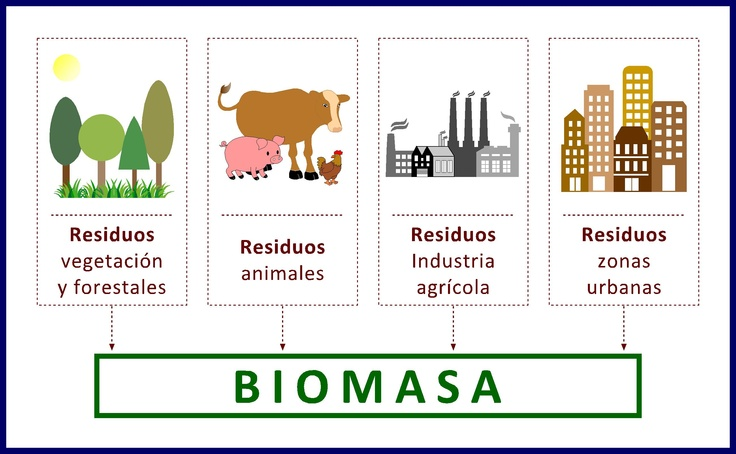
\includegraphics[width=\textwidth]{biomasa.jpg}
%  \caption{Distintas materias orgánicas.}
%  \label{fig:1}
%\end{figurebox}
%\end{wrapfigure}
%\end{center}
%\end{multicols}

%section{Atlas Global de Recurso Solar y Eólico}

%n 2013 se puso a disposición mundial el primer Atlas Global de recursos Solar y Eólico. El objetivo de la creación de este atlas es aumentar la conciencia en el planeta de generar energía limpia. La  Agencia Internacional de Energías Renovables (IRENA, por sus siglas en inglés) ha creado el primer Atlas Global de Energía Solar y Eólica de consulta online fue quien lideró este proyecto que podemos encontrar online aquí: \url{http://globalatlas.irena.org/}.

%ste atlas nos permite:
%begin{itemize}
%item Ver los mapas de recursos de los principales institutos técnicos en el mundo.
%item Acceso a las herramientas para la evaluación del potencial técnico de las energías renovables.
%\end{itemize}

%Mostramos a continuación algunos de los tipos de mapas que podemos observar con este atlas.

%\begin{figure}[ht!]
%\begin{center}
%\begin{figurebox}
%  \centering
%    \begin{subfigure}{\textwidth}
%  \centering
%   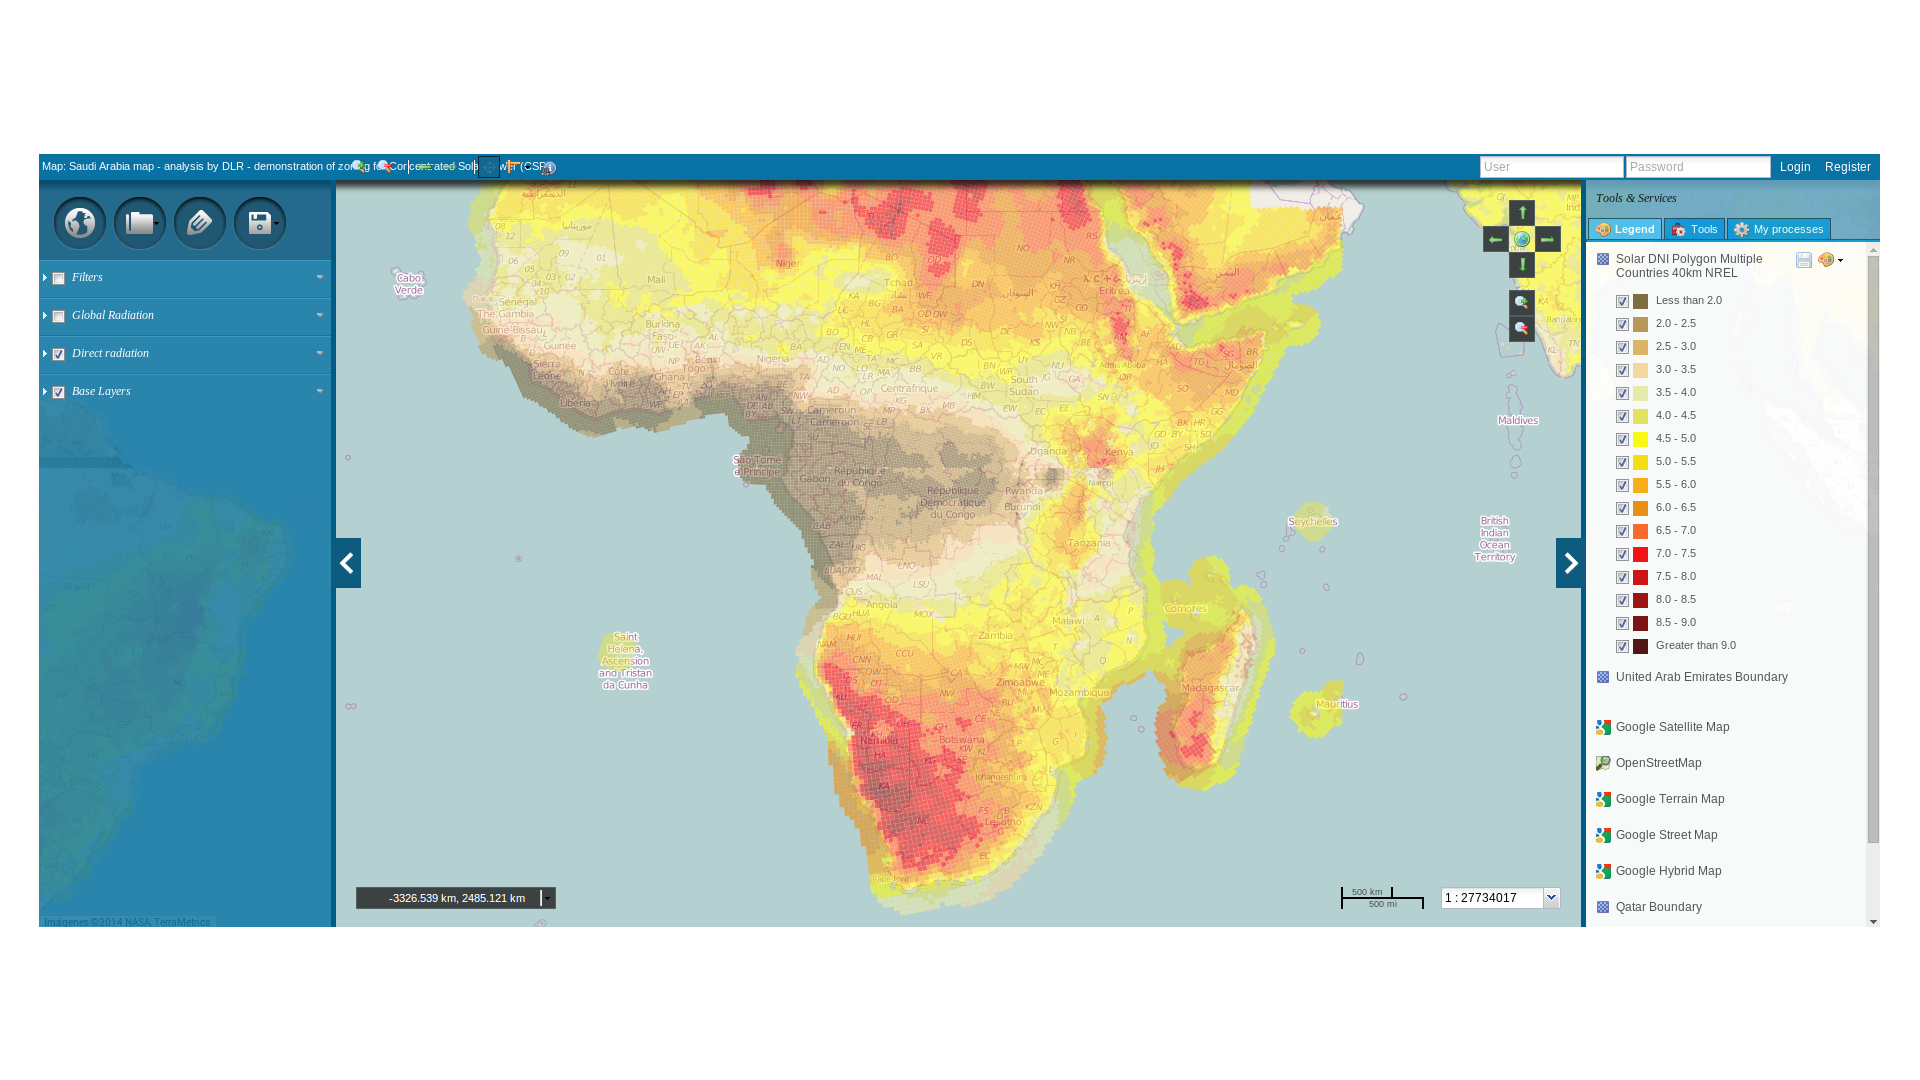
\includegraphics[scale=0.17]{radacion.png}

   %\caption{Contador}
%\end{subfigure}
% \begin{subfigure}{\textwidth}
%  \centering
%   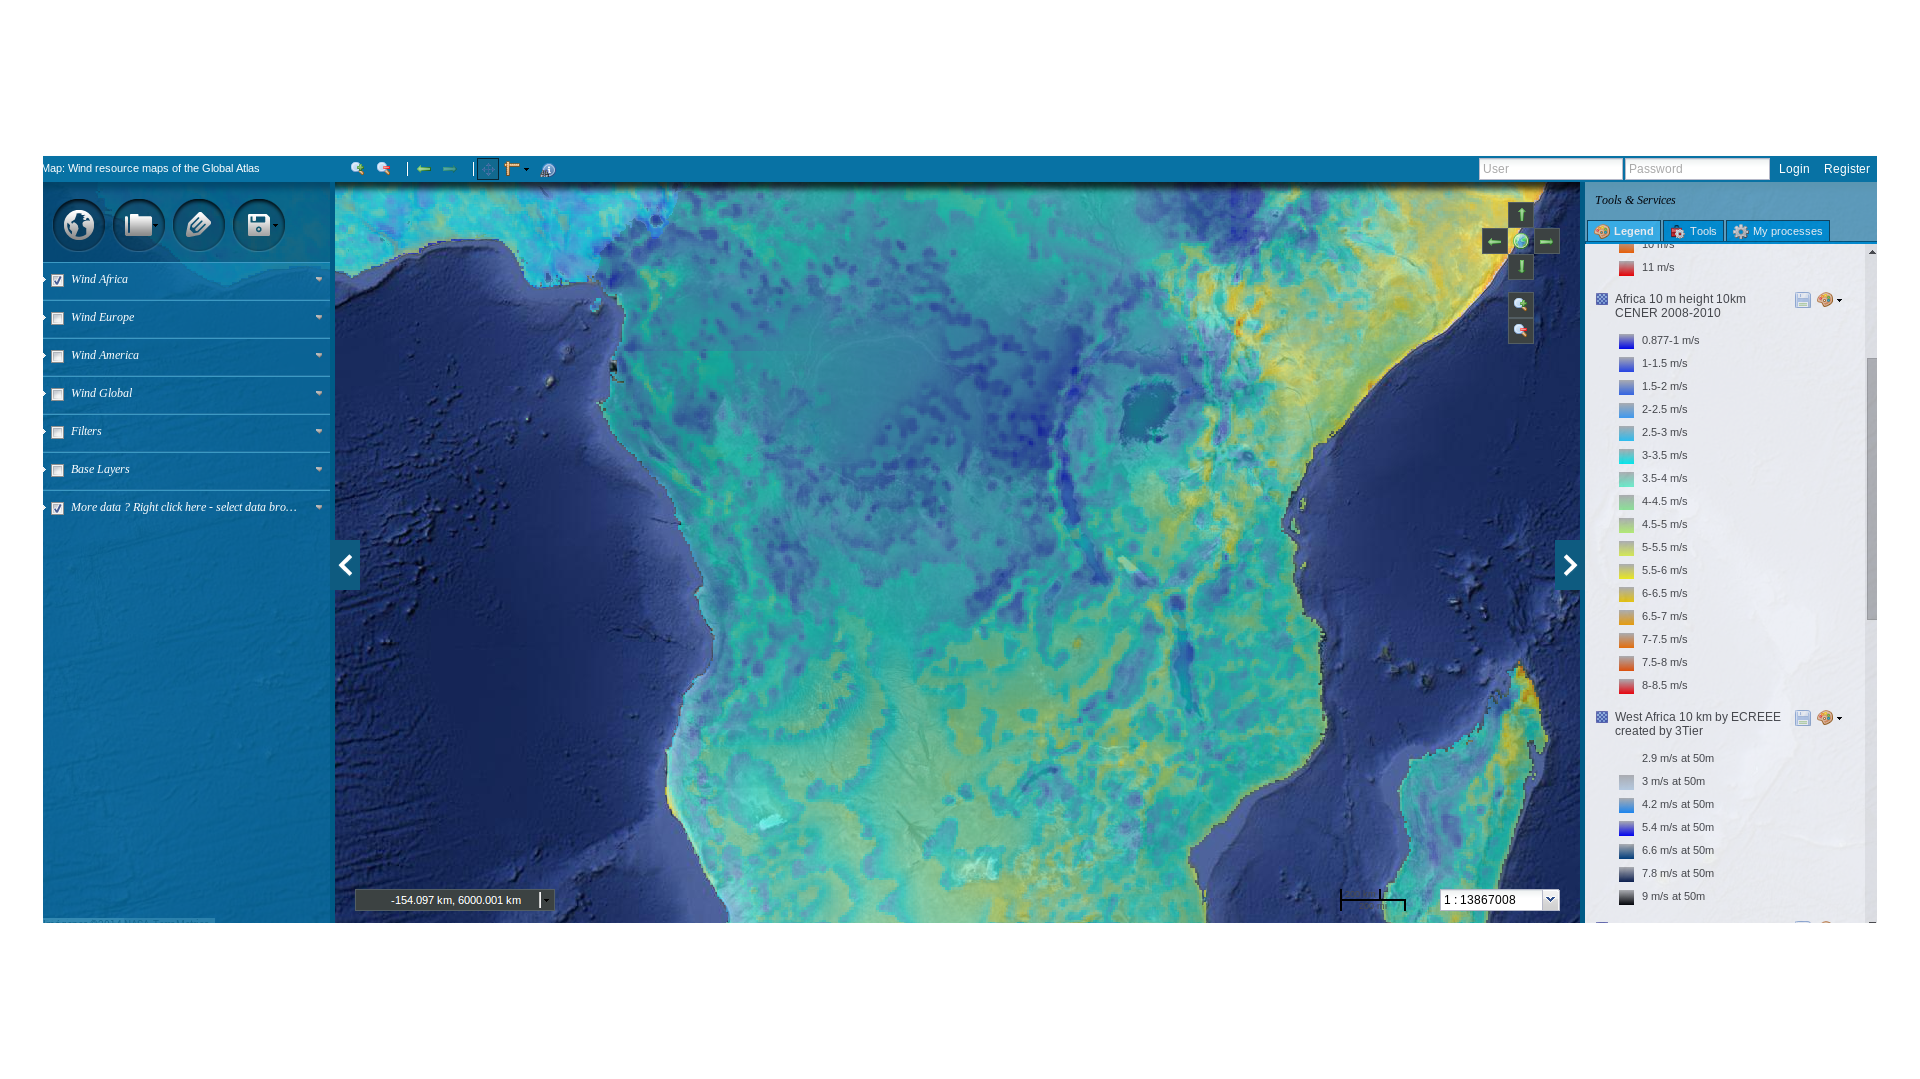
\includegraphics[scale=0.17]{vientoafrica.png}
   %\caption{PLC}
%\end{subfigure}
%begin{subfigure}{\textwidth}
%centering
% 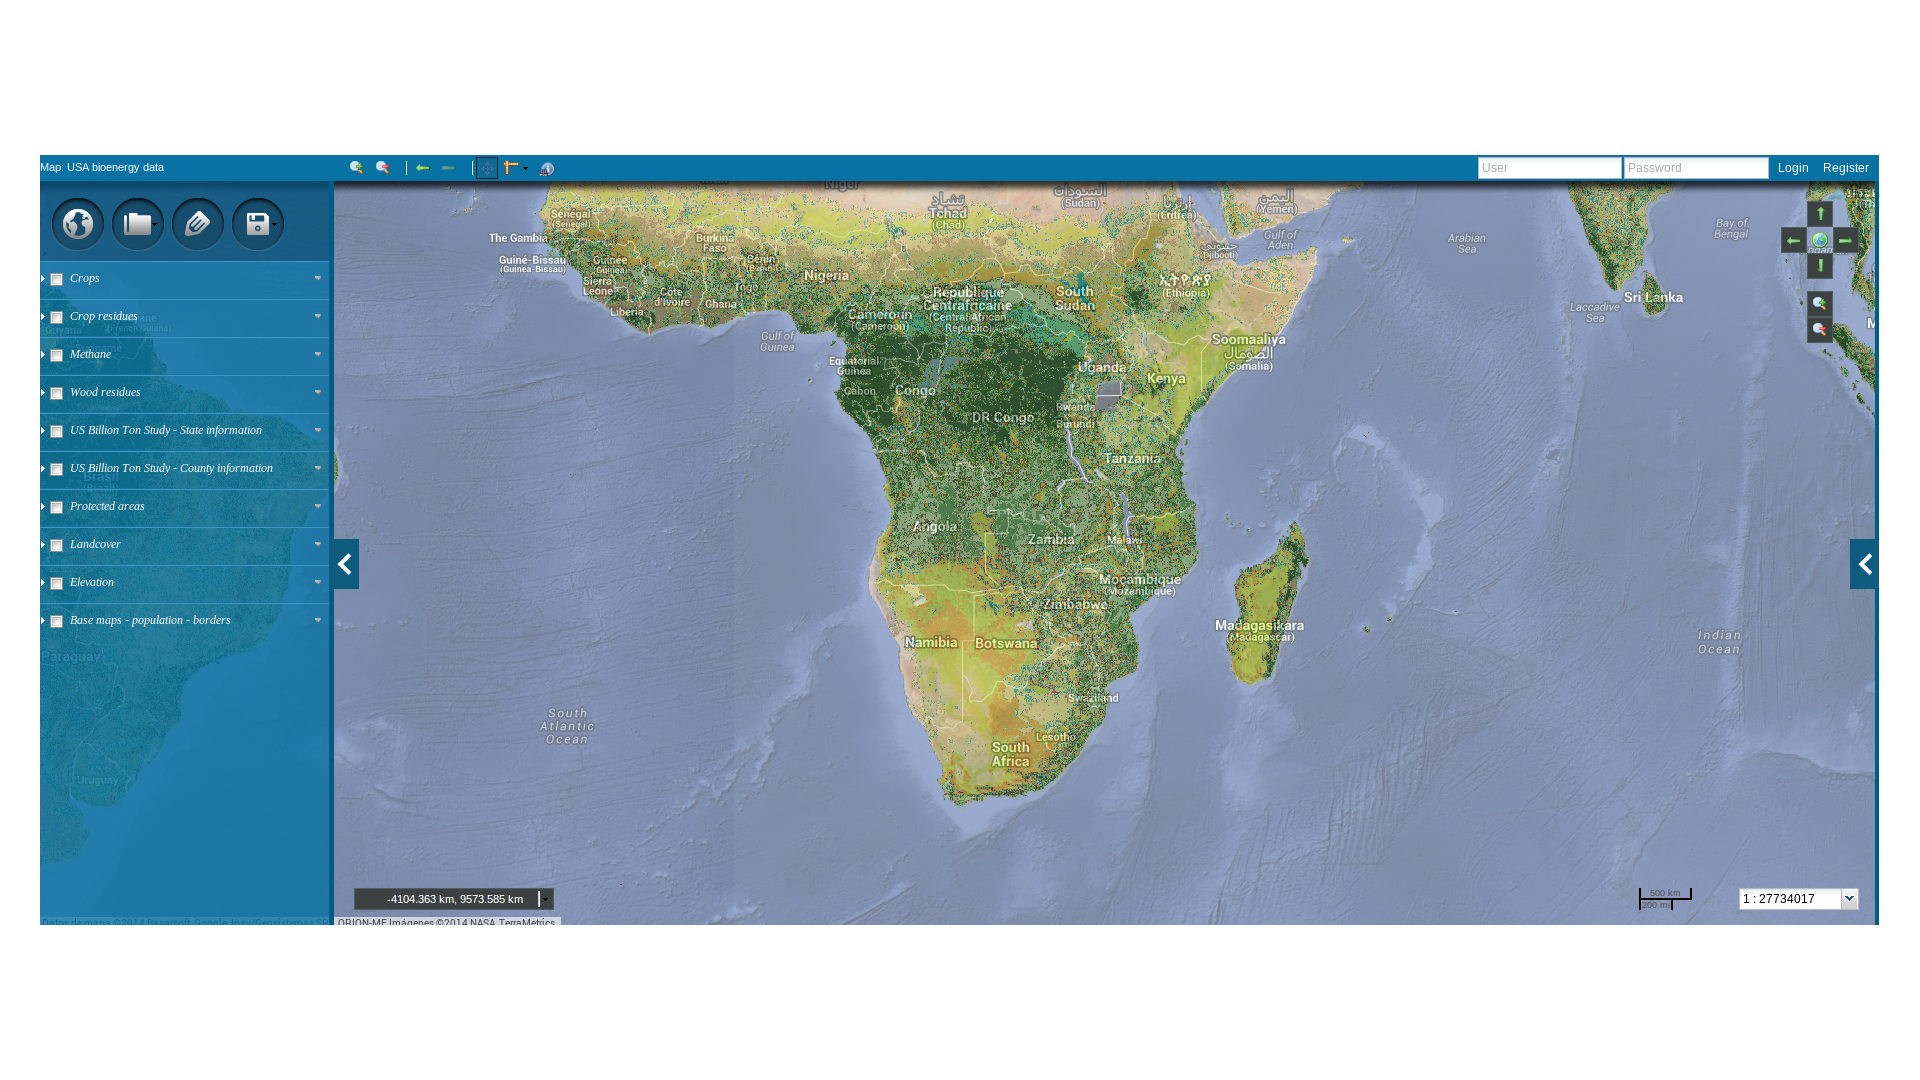
\includegraphics[scale=0.17]{biomateria.png}
  %\caption{Concentrador}
%\end{subfigure}
% \caption{De arriba a abajo: radiación, viento y bioenergía de África.} \label{fig:mapas}
%\end{figurebox}
%\end{center}
%\end{figure}

\end{multicols}

%\vspace{3.75cm} 
\noindent
%
\includegraphics[width=\textwidth,scale=0.5]{pubmm.png}

\newpage
%%% Local Variables: 
%%% mode: latex
%%% TeX-master: "novedades"
%%% End: 


